\documentclass[11pt,compress,t,notes=noshow, xcolor=table]{beamer}
\usepackage[]{graphicx}\usepackage[]{color}
% maxwidth is the original width if it is less than linewidth
% otherwise use linewidth (to make sure the graphics do not exceed the margin)
\makeatletter
\def\maxwidth{ %
  \ifdim\Gin@nat@width>\linewidth
    \linewidth
  \else
    \Gin@nat@width
  \fi
}
\makeatother

\definecolor{fgcolor}{rgb}{0.345, 0.345, 0.345}
\newcommand{\hlnum}[1]{\textcolor[rgb]{0.686,0.059,0.569}{#1}}%
\newcommand{\hlstr}[1]{\textcolor[rgb]{0.192,0.494,0.8}{#1}}%
\newcommand{\hlcom}[1]{\textcolor[rgb]{0.678,0.584,0.686}{\textit{#1}}}%
\newcommand{\hlopt}[1]{\textcolor[rgb]{0,0,0}{#1}}%
\newcommand{\hlstd}[1]{\textcolor[rgb]{0.345,0.345,0.345}{#1}}%
\newcommand{\hlkwa}[1]{\textcolor[rgb]{0.161,0.373,0.58}{\textbf{#1}}}%
\newcommand{\hlkwb}[1]{\textcolor[rgb]{0.69,0.353,0.396}{#1}}%
\newcommand{\hlkwc}[1]{\textcolor[rgb]{0.333,0.667,0.333}{#1}}%
\newcommand{\hlkwd}[1]{\textcolor[rgb]{0.737,0.353,0.396}{\textbf{#1}}}%
\let\hlipl\hlkwb

\usepackage{framed}
\makeatletter
\newenvironment{kframe}{%
 \def\at@end@of@kframe{}%
 \ifinner\ifhmode%
  \def\at@end@of@kframe{\end{minipage}}%
  \begin{minipage}{\columnwidth}%
 \fi\fi%
 \def\FrameCommand##1{\hskip\@totalleftmargin \hskip-\fboxsep
 \colorbox{shadecolor}{##1}\hskip-\fboxsep
     % There is no \\@totalrightmargin, so:
     \hskip-\linewidth \hskip-\@totalleftmargin \hskip\columnwidth}%
 \MakeFramed {\advance\hsize-\width
   \@totalleftmargin\z@ \linewidth\hsize
   \@setminipage}}%
 {\par\unskip\endMakeFramed%
 \at@end@of@kframe}
\makeatother

\definecolor{shadecolor}{rgb}{.97, .97, .97}
\definecolor{messagecolor}{rgb}{0, 0, 0}
\definecolor{warningcolor}{rgb}{1, 0, 1}
\definecolor{errorcolor}{rgb}{1, 0, 0}
\newenvironment{knitrout}{}{} % an empty environment to be redefined in TeX

\usepackage{alltt}
\newcommand{\SweaveOpts}[1]{}  % do not interfere with LaTeX
\newcommand{\SweaveInput}[1]{} % because they are not real TeX commands
\newcommand{\Sexpr}[1]{}       % will only be parsed by R



\usepackage[english]{babel}
\usepackage[utf8]{inputenc}

\usepackage{dsfont}
\usepackage{verbatim}
\usepackage{amsmath}
\usepackage{amsfonts}
\usepackage{bm}
\usepackage{csquotes}
\usepackage{multirow}
\usepackage{longtable}
\usepackage{booktabs}
\usepackage{enumerate}
\usepackage[absolute,overlay]{textpos}
\usepackage{psfrag}
\usepackage{algorithm}
\usepackage{algpseudocode}
\usepackage{eqnarray}
\usepackage{arydshln}
\usepackage{tabularx}
\usepackage{placeins}
\usepackage{tikz}
\usepackage{setspace}
\usepackage{colortbl}
\usepackage{mathtools}
\usepackage{wrapfig}
\usepackage{bm}
\usetikzlibrary{shapes,arrows,automata,positioning,calc,chains,trees, shadows}
\tikzset{
  %Define standard arrow tip
  >=stealth',
  %Define style for boxes
  punkt/.style={
    rectangle,
    rounded corners,
    draw=black, very thick,
    text width=6.5em,
    minimum height=2em,
    text centered},
  % Define arrow style
  pil/.style={
    ->,
    thick,
    shorten <=2pt,
    shorten >=2pt,}
}
\usepackage{subfig}


% Defines macros and environments
\input{../../style/common.tex}
% \input{common.tex}

%\usetheme{lmu-lecture}
\newcommand{\titlefigure}{figure_man/roc_metrics.png}
\newcommand{\learninggoals}{
\item Understand why accuracy is not an optimal performance measure for 
imbalanced labels
\item Understand the different measures computable from a confusion matrix
\item Be aware that each of these measures has a variety of names }
\usepackage{../../style/lmu-lecture}

\let\code=\texttt
\let\proglang=\textsf

\setkeys{Gin}{width=0.9\textwidth}

\title{Introduction to Machine Learning}
% \author{Bernd Bischl, Christoph Molnar, Daniel Schalk, Fabian Scheipl}
\institute{\href{https://compstat-lmu.github.io/lecture_i2ml/}{compstat-lmu.github.io/lecture\_i2ml}}
\date{}

\setbeamertemplate{frametitle}{\expandafter\uppercase\expandafter\insertframetitle}

\begin{document}

% This file loads R packages, configures knitr options and sets preamble.Rnw as parent file
% IF YOU MODIFY THIS, PLZ ALSO MODIFY setup.Rmd ACCORDINGLY...

% Defines macros and environments
\input{../../latex-math/basic-math.tex}
\input{../../latex-math/basic-ml.tex}
%! includes: evaluation-measures-classification

\lecturechapter{Evaluation: Measures for Binary Classification: ROC Measures}
\lecture{Introduction to Machine Learning}

% ------------------------------------------------------------------------------

% \begin{vbframe}{Imbalanced Binary Labels}
% 
% \begin{center}
% % FIGURE SOURCE: https://docs.google.com/drawings/d/1WERS9WXwS4zla86fk6ESQkskNN1WZMI1YCPprnp0Ew0/edit?usp=sharing
% \includegraphics[width=.9\textwidth]{figure_man/imbalanced.pdf}\\
% Classify all as \enquote{no disease} (green) $\rightarrow$ high accuracy.
% 
% \lz
% 
% \textbf{Accuracy Paradox}
% \end{center}
% 
% \end{vbframe}

% ------------------------------------------------------------------------------

% \begin{vbframe}{Imbalanced Costs}
% 
% \begin{center}
% % FIGURE SOURCE: https://docs.google.com/drawings/d/1GlmMqzpeNHU_rtPFIrJMlY9Iz6XexvHEwTl3dNYKyQU/edit?usp=sharing
% \includegraphics[width=.3\textwidth]{figure_man/imbalanced-costs.pdf}\\
% Classify incorrectly as \enquote{no disease} $\rightarrow$ very high cost
% 
% \end{center}
% 
% \end{vbframe}

% ------------------------------------------------------------------------------

\begin{vbframe}{class imbalance}

\begin{itemize}
 \item Consider a binary classifier for diagnosing a serious medical 
 condition.
 \item Here, label distribution is often \textbf{imbalanced}, i.e, not many 
 people have the disease.
 \item Evaluating on error rates is often inappropriate for scenarios with 
 imbalanced labels:
 \begin{itemize}
   \item Assume that only 0.5\,\% of 1000 patients have the disease.
   \item Always returning \enquote{no disease} has an error rate of 0.5\,\%, 
   corresponding to very high accuracy.
   \item However, this sends all sick patients home, which is the worst 
   possible system -- even classifying everyone as \enquote{disease} might be 
   better (depending on the treatment).
 \end{itemize}
 \item This problem is known as the \textbf{accuracy paradox}.
\end{itemize}

Classifying all observations as \enquote{no disease} (green) yields top 
accuracy simply because the \enquote{disease} occurs so rarely 
$\rightarrow$ accuracy paradox.

\lz

\begin{center}
  % FIGURE SOURCE: https://docs.google.com/drawings/d  /1WERS9WXwS4zla86fk6ESQkskNN1WZMI1YCPprnp0Ew0/edit?usp=sharing
  \includegraphics[width=0.7\textwidth]{figure_man/imbalanced.pdf}
\end{center}

\end{vbframe}
 
% ------------------------------------------------------------------------------

\begin{vbframe}{imbalanced costs}
 
\begin{itemize}
  \item Another point of view is \textbf{imbalanced costs}.
  \item In our example, classifying a sick patient as healthy should incur a 
  much higher loss then classifying a healthy patient as sick.
  \item The costs depend a lot on what happens next: we can likely assume that 
  our system is some type of screening filter, and often the next step after 
  labeling someone as sick might be a more invasive, expensive, but also  more 
  reliable test for the disease.
  \item Erroneously subjecting someone to this step is undesirable 
  (psychological, economic, medical expense), but sending someone home to get 
  worse or die seems is much more so.
  \item Such situations not only arise under label imbalance, but also when 
  costs differ (even though classes might be balanced).
  \item We could see this as imbalanced costs of misclassification, rather than 
  imbalanced labels; both situations are tightly connected.
\end{itemize}

\framebreak

\lz

\begin{minipage}[c]{0.65\textwidth}
  \raggedright
  \textbf{Imbalanced costs: } classifying incorrectly as \enquote{no disease} 
  incurs very high cost.
\end{minipage}%
\begin{minipage}[c]{0.35\textwidth}
  \centering
  \includegraphics[trim = 0 0 0 10, clip, width=0.4\textwidth]
  {figure_man/imbalanced-costs.pdf}
\end{minipage}

\lz

\begin{itemize}
  \item Problem: if we were able to specify costs precisely, we could evaluate 
  or even optimize on them.
  \item This important subfield of ML is called \textbf{cost-sensitive 
  learning}, which we will not cover in this lecture unit.
  \item Unfortunately, users tend to find it notoriously hard to come up with 
  precise cost figures in imbalanced scenarios.
  \item Evaluating \enquote{from different perspectives}, with multiple metrics, 
  often helps to get a first impression of system quality.
\end{itemize}
 
\end{vbframe}
 
% ------------------------------------------------------------------------------
 
 % \begin{vbframe}{Binary Classifiers and Costs}
 % \begin{itemize}
 %   \item Problem is: If we could specify costs precisely, we could evaluate against them, we might even optimize our model for them
 %   \item This important subfield of ML is called \textbf{cost-sensitive learning}, which we will not cover in this lecture unit
 %   \item Unfortunately, users often have a notoriously hard time to come up with precise cost numbers in imbalanced scenarios
 %   \item Evaluating "from different perspectives", with multiple metrics, often helps, especially to get a first impression
 %     of the quality of the system
 % \end{itemize}
 % \end{vbframe}

% ------------------------------------------------------------------------------

\begin{frame}{ROC Analysis}

\begin{itemize}
  \item \textbf{ROC analysis} is a subfield of ML which studies the evaluation 
  of binary prediction systems.
  \item ROC stands for \enquote{receiver operating characteristics} and was 
  initially developed by electrical engineers and radar engineers during World 
  War II for detecting enemy objects in battlefields -- still has the funny 
  name.
\end{itemize}

\lz

\begin{center}
\includegraphics[width=.4\textwidth]{figure_man/receiver_operator.jpg}
{\tiny \url{http://media.iwm.org.uk/iwm/mediaLib//39/media-39665/large.jpg}}
\end{center}

\end{frame}

% ------------------------------------------------------------------------------

%  \begin{vbframe}{Confusion Matrix and ROC Metrics}
%  \begin{itemize}
%    \item From now on, we will call one class "positive", one "negative" and 
%    their respective sizes $n_+$ and $n_-$.
%    \item The positive class is the more important, often smaller one.
%    \item We represent all predictions in a confusion matrix and count correct 
%    and incorrect class assignments
%    \item False Positive means: We assigned "positive", but were wrong
%  \end{itemize}
% % % FIGURE SOURCE: No source
%  \includegraphics[width=0.7\textwidth]{figure_man/roc-confmatrix1.png}
%  \end{vbframe}

% ------------------------------------------------------------------------------

% \begin{vbframe}{Confusion Matrix}
% 
% \begin{center}
% \small
% \renewcommand{\arraystretch}{1.5}
% \begin{tabular}{cc||cc}
%     & & \multicolumn{2}{c}{\bfseries True Class $y$}  \\
%     & & $+$ & $-$  \\ 
%     \hline \hline
%     \bfseries Pred.     & $+$ & TP & FP\\
%               $\yh$ & $-$ & FN & TN\\ 
% \end{tabular}
% \renewcommand{\arraystretch}{1}
% \end{center}
% 
% \begin{itemize}
%   \item $+$: \enquote{positive} class
%   \item $-$: \enquote{negative} class
%   \item $\np$: number of observations in $+$
%   \item $\nn$: number of observations in $-$
% \end{itemize}
% \end{vbframe}

% ------------------------------------------------------------------------------

\begin{vbframe}{Labels: ROC Metrics}
From the confusion matrix (binary case), we can calculate "ROC" metrics.

% % FIGURE SOURCE: No source
% \includegraphics[width=0.7\textwidth]{figure_man/roc-confmatrix2.png}

% \begin{center}
% \small
% \begin{tabular}{cc|>{\centering\arraybackslash}p{7em}>{\centering\arraybackslash}p{8em}|>{\centering\arraybackslash}p{8em}}
%     & & \multicolumn{2}{c}{\bfseries True Class $y$} & \\
%     & & $+$ & $-$ & \\
%     \hline
%     \bfseries Pred.     & $+$ & True Positive (TP)  & False Positive (FP) & Positive Predictive Value (PPV) = $\frac{\text{TP}}{\text{TP} + \text{FP}}$\\
%               $\hat{y}$ & $-$ & False Negative (FN) & True Negative (TN) & Negative Predictive Value (NPV) = $\frac{\text{TN}}{\text{FN} + \text{TN}}$\\
%     \hline
%     & & TPR = $\frac{\text{TP}}{\text{TP} + \text{FN}}$ & TNR = $\frac{\text{TN}}{\text{FP} + \text{TN}}$ & Accuracy = $\frac{\text{TP}+ \text{TN}}{\text{TOTAL}}$
% \end{tabular}
% \end{center}

\begin{center}
\small
\renewcommand{\arraystretch}{1.5}
\begin{tabular}{cc||cc|c}
    & & \multicolumn{2}{c|}{\bfseries True Class $y$} & \\
    & & $+$ & $-$ & \\ 
    \hline \hline
    \bfseries Pred.     & $+$ & TP & FP & $\rho_{PPV} = \frac{\text{TP}}{\text{TP} + \text{FP}}$\\
              $\yh$ & $-$ & FN & TN & $\rho_{NPV} = \frac{\text{TN}}{\text{FN} + \text{TN}}$\\
    \hline
    & & $\rho_{TPR} = \frac{\text{TP}}{\text{TP} + \text{FN}}$ & $\rho_{TNR} = \frac{\text{TN}}{\text{FP} + \text{TN}}$ & $\rho_{ACC} = \frac{\text{TP}+ \text{TN}}{\text{TOTAL}}$
\end{tabular}
\renewcommand{\arraystretch}{1}
\end{center}

\begin{itemize}
  \small
  \item True positive rate $\rho_{TPR}$: how many of the true 1s did we predict 
  as 1?
  \item True Negative rate $\rho_{TNR}$: how many of the true 0s did we predict 
  as 0?
  \item Positive predictive value $\rho_{PPV}$: if we predict 1, how likely is 
  it a true 1?
  \item Negative predictive value $\rho_{NPV}$: if we predict 0, how likely is 
  it a true 0?
  \item Accuracy $\rho_{ACC}$: how many instances did we predict correctly?
\end{itemize}
\end{vbframe}

% ------------------------------------------------------------------------------

\begin{vbframe}{Labels: ROC Metrics}

Example:

\begin{center}
  % FIGURE SOURCE: No source
  \includegraphics[width=\textwidth]{figure_man/roc-confmatrix-example.png}
\end{center}

\end{vbframe}

% ------------------------------------------------------------------------------

\begin{vbframe}{More metrics and alternative terminology}

Unfortunately, for many concepts in ROC, 2-3 different terms exist.

\begin{center}
% FIGURE SOURCE: https://en.wikipedia.org/wiki/F1_score#Diagnostic_testing
\includegraphics[width=0.95\textwidth]{figure_man/roc-confmatrix-allterms.png}
\end{center}
\href{https://en.wikipedia.org/wiki/F1_score#Diagnostic_testing}{\beamergotobutton{Clickable version/picture source}} $\phantom{blablabla}$
\href{https://upload.wikimedia.org/wikipedia/commons/0/0e/DiagnosticTesting_Diagram.svg}{\beamergotobutton{Interactive diagram}}
\end{vbframe}

% ------------------------------------------------------------------------------

\begin{vbframe}{Labels: $F_1$ Measure}

\small

\begin{itemize}
  \item It is difficult to achieve high \textbf{positive predictive value} and 
  high \textbf{true positive rate} simultaneously.
   \item A classifier predicting more positive will be more 
   sensitive (higher $\rho_{TPR}$), but it will also tend to give more 
   \textit{false} positives (lower $\rho_{TNR}$, lower $\rho_{PPV}$).
   \item A classifier that predicts more negatives will be more precise 
   (higher $\rho_{PPV}$), but it will also produce more \textit{false} negatives 
   (lower $\rho_{TPR}$).
 \end{itemize}

The \textbf{$F_1$ score} balances two conflicting goals:\\%[.5em]
\begin{enumerate}
 \item Maximizing positive predictive value
 \item Maximizing true positive rate \\%[.5em]
\end{enumerate}

$\rho_{F_1}$ is the harmonic mean of $\rho_{PPV}$ and $\rho_{TPR}$:
$$\rho_{F_1} = 2 \cdot \cfrac{\rho_{PPV} \cdot \rho_{TPR}}{\rho_{PPV} + 
\rho_{TPR}}$$

Note that this measure still does not account for the number of true
negatives.

\framebreak

\normalsize

\begin{minipage}[c]{0.5\textwidth}
  \small
  $F_1$ score for different combinations of $\rho_{PPV}$ \& $\rho_{TPR}$. \\
  $\rightarrow$ Tends more towards the lower of the two combined values.
\end{minipage}%
\begin{minipage}[c]{0.5\textwidth}
  \centering
  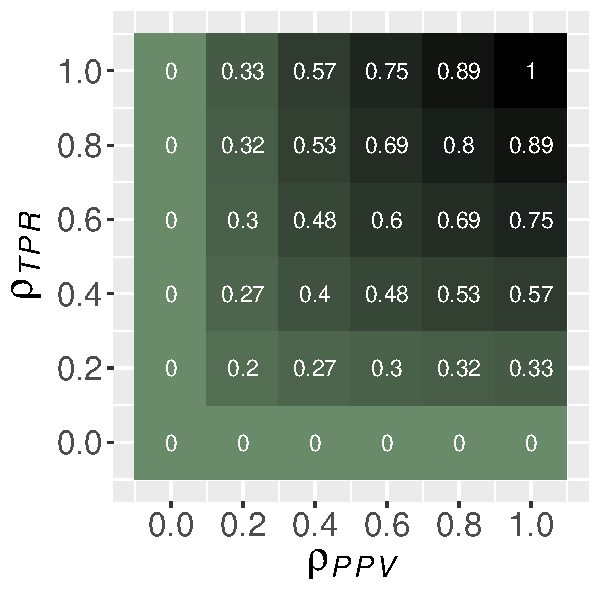
\includegraphics[width=0.8\textwidth]{figure/eval_mclass_roc.pdf}
\end{minipage}

% Tabulated $F_1$-Score for different TPR (rows) and PPV (cols) combinations:
% \begin{knitrout}\scriptsize
% \definecolor{shadecolor}{rgb}{0.969, 0.969, 0.969}\color{fgcolor}
% 
% 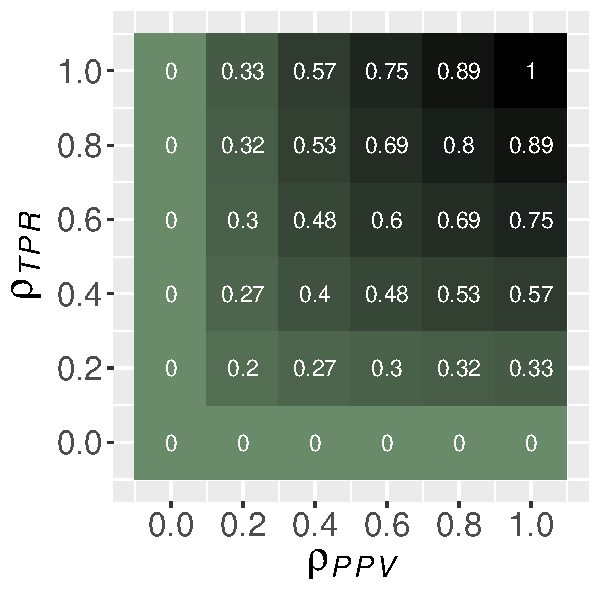
\includegraphics[width=0.5\textwidth]{figure/eval_mclass_roc.pdf}
% 
% \end{knitrout}
% $\rightarrow$ Tends more towards the lower of the two combined values.

\begin{itemize}
  \item A model with $\rho_{TPR} = 0$ (no positive instance predicted as 
  positive) or 
  $\rho_{PPV} = 0$ (no true positives among the predicted) has $\rho_{F_1} = 0$.
  \item Always predicting \enquote{negative}: $\rho_{F_1} = 0$.
  \item Always predicting \enquote{positive}: $\rho_{F_1} = 2 \cdot \rho_{PPV} / 
  (\rho_{PPV} + 1) = 2 \cdot \np / (\np + n)$,\\ 
  which will be small when the size of the positive class $\np$ is small.
\end{itemize}

\end{vbframe}

% ------------------------------------------------------------------------------

\begin{vbframe}{which metric to use?}

\begin{itemize}
  \footnotesize
  \item As we have seen, there is a plethora of methods. \\
  $\rightarrow$ This leaves practitioners with the question of which to use.
  \item Consider a small benchmark study.
  \begin{itemize}
    \footnotesize
    \item We let $k$-NN, logistic regression, a classification tree, and a random 
    forest compete on classifying the \texttt{credit risk} data.
    \item The data consist of 1000 observations of borrowers' financial 
    situation and their creditworthiness (good/bad) as target.
    \item Predicted probabilities are thresholded at 0.5 for the positive class.
    % \item We benchmark our learners on accuracy, AUC, $F_1$, precision, recall 
    % and specificity.
    \item Depending on the metric we use, learners are ranked differently 
    according to performance (value of respective performance measure in 
    parentheses):
  \end{itemize}
\end{itemize}

\begin{center}
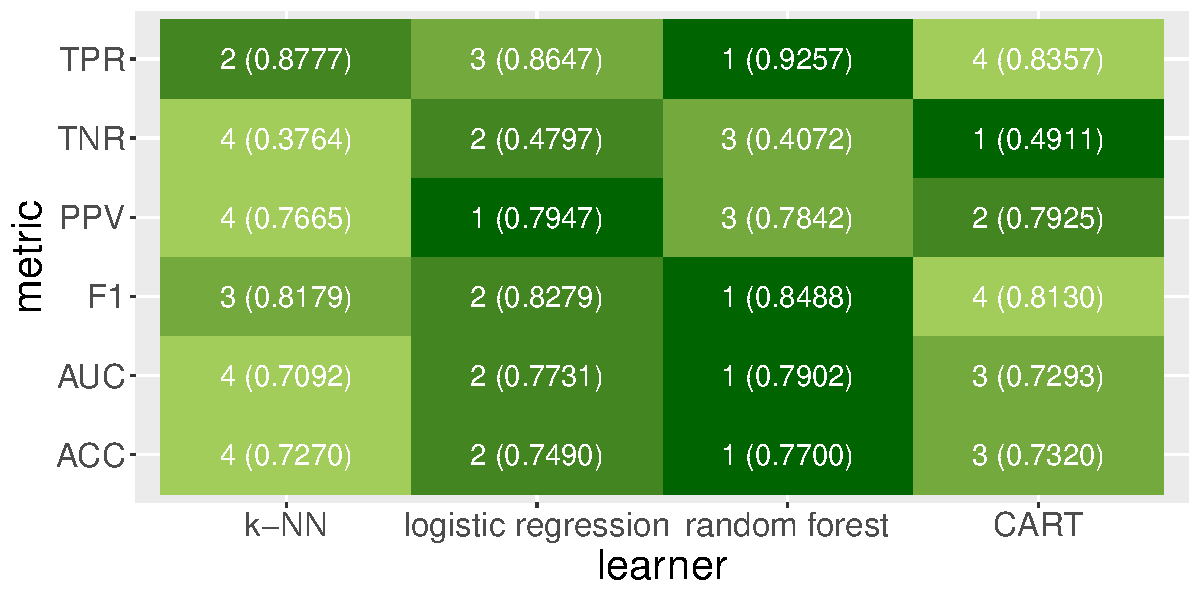
\includegraphics[width=0.6\textwidth]{figure/eval_mclass_benchmark.pdf}
\end{center}

\framebreak

\begin{itemize}
  \item We need not expect overly large discrepancies in general, but neither 
  will we always see an unambiguous picture. 
  \item Different metrics emphasize different aspects of performance. \\
  $\rightarrow$ The choice should be made in the domain context.
  \item For practitioners it is vital to understand what should be 
  evaluated exactly, and which measure is appropriate.  
  \begin{itemize}
    \item Regarding credit risk, for instance, defaults are to be avoided, but 
    not at all cost.
    \item The bank must undertake a certain risk to remain profitable, so a more 
    balanced measure such as the $F_1$ score might be in order.
    \item On the other hand, a system detecting weapons at an airport should be 
    able to achieve very high true positive rates, even if this comes at the 
    expense of some false alarms.
  \end{itemize}
\end{itemize}

\end{vbframe}

% ------------------------------------------------------------------------------

\endlecture

\end{document}
